%%%%%%%%%%%%%%%%%%%%%%%%%%%%%%%%%%%%%%%%%%%%%%%%%%%%%%%%%
% KONFIGURATIONEN
%%%%%%%%%%%%%%%%%%%%%%%%%%%%%%%%%%%%%%%%%%%%%%%%%%%%%%%%%

\documentclass[
    12pt,               
    a4paper,        
    ngerman            
]{scrartcl}

\usepackage[utf8]{inputenc}            
\usepackage[ngerman]{babel}            
\usepackage{geometry}                   
\usepackage{amsmath}                   
\usepackage{amssymb}                   
\usepackage{graphicx}                   
\usepackage{parskip}
\usepackage{csquotes}
\usepackage{xcolor}
\usepackage[
    pdftitle={Abschlussbericht DABI2}, 
    pdfauthor={Wiederstein / Jan-David},
    hidelinks
]{hyperref}                             
\usepackage{microtype}                 
\usepackage[backend=biber]{biblatex}  
\addbibresource{literatur.bib}        

\geometry{left=2.5cm, right=2.5cm, top=2.5cm, bottom=2.5cm}

\pagestyle{headings} 

%%%%%%%%%%%%%%%%%%%%%%%%%%%%%%%%%%%%%%%%%%%%%%%%%%%%%%%%%
% TITELSEITE
%%%%%%%%%%%%%%%%%%%%%%%%%%%%%%%%%%%%%%%%%%%%%%%%%%%%%%%%%

\title{Architektur und Analyse zum Trinkgeldverhalten}
\author{Keanu Nachname, Andro Nachname, Benjamin Nachname, Jan-David Wiederstein}
\date{\today}

\begin{document}

\begin{titlepage}
    \centering
    
    \vfill 
    
\includegraphics[width=0.8\textwidth]{logo.png}\par\vspace{1cm}
    
    {\Huge \bfseries Architektur und Analyse zum Trinkgeldverhalten\par} 
    
    \vspace{0.5cm}
    
    {\LARGE Abschlussbericht Semesterprojekt\par} 

    \vspace{0.5cm}

    {\large \today\par} 

    \vspace{1.5cm} 

    \large
    \begin{tabular}{l l}
        Keanu Sky Heitzler & Matrikel-Nr.: 90672 \\
        Andro Oraha & Matrikel-Nr.: 81542 \\
        Benjamin Bartel & Matrikel-Nr.: 90708 \\
        Jan-David Wiederstein & Matrikel-Nr.: 88219 \\
    \end{tabular}

    \vfill

    {\normalsize
    Hochschule Karlsruhe \\
    Data Science B.Sc. \\
    Modul: Datenanalyse und Business Intelligence 2 \\
    Dozent: Prof. Dr. Küppers und Prof. Dr. Hofmann
    \par}
    
\end{titlepage}

%%%%%%%%%%%%%%%%%%%%%%%%%%%%%%%%%%%%%%%%%%%%%%%%%%%%%%%%%
% ABSTRACT
%%%%%%%%%%%%%%%%%%%%%%%%%%%%%%%%%%%%%%%%%%%%%%%%%%%%%%%%%

\begin{abstract}
    \noindent
    \section*{Abstract}
    Um die Entwicklung datengetriebener Anwendungsfälle zu ermöglichen, ohne die Stabilität des operativen Tagesgeschäfts zu gefährden, wurde im Rahmen dieses Projekts eine moderne, an die Kappa-Architektur angelehnte Datenarchitektur konzipiert. Anhand des Kunden-Use-Cases einer fairen Zuteilung von Bestellungen mit hoher Trinkgeldwahrscheinlichkeit wird der Bedarf der Fachanalysten an performantem Datenzugriff verdeutlicht. Die implementierte Lösung nutzt Change Data Capture (CDC) via Debezium, um Datenänderungen aus der produktiven OLTP-Datenbank nahezu in Echtzeit und mit minimaler Last abzugreifen und über eine zentrale Streaming-Plattform (Kafka) zu verteilen. Das Ergebnis ist ein S3-kompatibler Data Lake als Rohdatenspeicher sowie ein darauf aufbauendes, mittels dbt transformiertes Data Warehouse in ClickHouse. Diese entkoppelte Architektur stellt Analysten die benötigten Daten in Form von Fakten- und Dimensionstabellen zur Verfügung und schützt zugleich die Integrität und Verfügbarkeit der kritischen Geschäftsanwendungen.
\end{abstract}

%%%%%%%%%%%%%%%%%%%%%%%%%%%%%%%%%%%%%%%%%%%%%%%%%%%%%%%%%
% INHALTSVERZEICHNIS
%%%%%%%%%%%%%%%%%%%%%%%%%%%%%%%%%%%%%%%%%%%%%%%%%%%%%%%%%

\newpage 
\tableofcontents
\newpage

%%%%%%%%%%%%%%%%%%%%%%%%%%%%%%%%%%%%%%%%%%%%%%%%%%%%%%%%%
% KAPITEL 1
%%%%%%%%%%%%%%%%%%%%%%%%%%%%%%%%%%%%%%%%%%%%%%%%%%%%%%%%%

\section{Einleitung}
Unternehmen stehen zunehmend vor der Herausforderung, ihre operativen Daten (OLTP) für komplexe Analysen zu nutzen, ohne die Stabilität der produktiven Systeme zu gefährden. Direkte analytische Abfragen bergen erhebliche Performance-Risiken für das Kerngeschäft. Die zentrale Fragestellung dieser Arbeit ist daher, wie eine entkoppelte Datenarchitektur gestaltet werden kann, die sichere und performante Analysen ermöglicht.

Als treibender Anwendungsfall dient ein fiktiver Lieferdienst, der zur Steigerung der Mitarbeiterzufriedenheit die Trinkgeldwahrscheinlichkeit von Bestellungen analysieren möchte. Dies erfordert einen flexiblen Zugriff auf historische Bestelldaten, ohne das Tagesgeschäft zu beeinträchtigen.

Um diese Anforderung zu erfüllen, wird eine moderne, an die Kappa-Architektur angelehnte Datenplattform konzipiert und prototypisch umgesetzt. Der Ansatz basiert auf Change Data Capture (CDC) via Debezium, um Datenänderungen aus der PostgreSQL-Quelldatenbank in Echtzeit zu erfassen und über Apache Kafka als Ereignisstrom zu verteilen. Diese Events werden in einem S3-basierten Data Lake persistiert und durch einen orchestrierten Prozess in ein analytisches ClickHouse Data Warehouse geladen. Dort transformiert das Werkzeug dbt die Rohdaten in ein analysefreundliches Sternschema. Die resultierende Architektur gewährleistet die entscheidende Entkopplung von operativen und analytischen Systemen und schafft eine skalierbare, stets aktuelle Datenbasis.

Dieser Bericht dokumentiert den Weg von der Konzeption über die technische Implementierung bis zur Validierung der Ergebnisse. Er schließt mit einer kritischen Reflexion und einem Ausblick auf mögliche Erweiterungen.
%%%%%%%%%%%%%%%%%%%%%%%%%%%%%%%%%%%%%%%%%%%%%%%%%%%%%%%%%
% KAPITEL 2
%%%%%%%%%%%%%%%%%%%%%%%%%%%%%%%%%%%%%%%%%%%%%%%%%%%%%%%%%
\section{Grundlagen und verwendete Technologien}

\subsection{Architekturmuster für Datenplattformen}
\label{sec:architekturmuster}
Um Daten aus OLTP-Systemen für OLAP-Zwecke nutzbar zu machen, hat sich unter anderem ein Architekturmuster etabliert.

\paragraph{Kappa-Architektur} Ein moderneres, vereinfachtes Muster, das auf die Batch-Ebene verzichtet. Die Grundidee ist, alle Daten – ob historisch oder in Echtzeit – als einen einzigen, unveränderlichen Ereignisstrom (Stream) zu behandeln. Die gesamte Verarbeitung erfolgt in einer einzigen Pipeline. Als \textit{Source of Truth} dient ein verteiltes Log-System wie Apache Kafka, das die Ereignisse für einen langen Zeitraum speichern kann. Muss eine Berechnung neu durchgeführt werden, werden die Daten einfach erneut aus dem Stream gelesen. Die in diesem Projekt umgesetzte Architektur ist stark an diesem Muster angelehnt.

\subsection{Change Data Capture (CDC)}
\label{sec:cdc}
Change Data Capture ist eine Technik, um Datenänderungen (INSERTS, UPDATES, DELETES) in einer Datenbank in Echtzeit zu identifizieren und zu erfassen. Anstatt die Datenbank periodisch mit Massen-Abfragen zu belasten (Batch-Export), liest CDC die Änderungen direkt aus dem Transaktionsprotokoll der Datenbank. Dieser Ansatz hat entscheidende Vorteile:
\begin{itemize}
    \item \textbf{Minimale Last:} Die Belastung für die Quelldatenbank ist äußerst gering.
    \item \textbf{Echtzeit-Fähigkeit:} Änderungen werden sofort erfasst und können weitergeleitet werden.
    \item \textbf{Vollständigkeit:} Alle Änderungen, auch Löschungen, werden zuverlässig erfasst.
\end{itemize}
\textbf{Debezium} ist ein weit verbreitetes Open-Source-Werkzeug, das als Konnektor für Apache Kafka fungiert und CDC für eine Vielzahl von Datenbanken, darunter PostgreSQL, ermöglicht.

\subsection{Kernkomponenten der implementierten Architektur}
\label{sec:kernkomponenten}

\paragraph{Apache Kafka} Eine verteilte Streaming-Plattform, die als zentrales Nervensystem der Architektur dient. Kafka nimmt die von Debezium erzeugten Datenänderungs-Events entgegen, speichert sie in themenspezifischen Kanälen (Topics) und stellt sie verschiedenen Konsumenten zuverlässig und skalierbar zur Verfügung.

\paragraph{Data Lake} Ein zentraler Speicherort für Rohdaten in ihrem nativen Format. Im Gegensatz zum hochstrukturierten Data Warehouse können in einem Data Lake strukturierte, semi-strukturierte und unstrukturierte Daten abgelegt werden. In diesem Projekt dient ein S3-kompatibler \textbf{Minio}-Bucket als Data Lake, in dem die Kafka-Events als Parquet-Dateien persistiert werden. Das spaltenorientierte Parquet-Format ist für analytische Abfragen besonders effizient.

\paragraph{Data Warehouse (DWH)} Ein zentraler, themenorientierter und historisierter Datenspeicher, der speziell für analytische Abfragen optimiert ist. Die Daten im DWH sind bereinigt, transformiert und in einem leicht verständlichen Datenmodell (z.B. Sternschema) strukturiert.

\subsection{Werkzeuge im modernen Data-Stack}
\label{sec:werkzeuge}

\paragraph{dbt (data build tool)} Ein Transformationswerkzeug, das es ermöglicht, Daten direkt im Data Warehouse mithilfe von SQL zu modellieren. dbt bringt Software-Engineering-Praktiken wie Versionierung, Modularisierung und automatisierte Tests in die Analytics-Welt. Es liest Rohdaten aus einer Quelle, transformiert sie und lädt sie als Fakten- und Dimensionstabellen in das DWH.

\paragraph{ClickHouse} Ein quelloffenes, spaltenorientiertes Datenbankmanagementsystem (DBMS), das für Online Analytical Processing (OLAP) konzipiert wurde. ClickHouse ist auf extrem hohe Performance bei der Verarbeitung von analytischen Echtzeit-Abfragen auf sehr großen Datenmengen spezialisiert. Im Gegensatz zu prozessinternen Datenbanken operiert ClickHouse als eigenständiger, hoch skalierbarer Server, was den Einsatz in produktiven und verteilten Architekturen ermöglicht. In diesem Projekt dient es als zentrale Data-Warehouse-Technologie.

\paragraph{Prefect} Ein modernes Workflow-Orchestration-Framework, geschrieben in Python. Es wird verwendet, um den gesamten Datenfluss zu definieren, zu planen und zu überwachen – vom Abholen der Daten aus Kafka über die Speicherung im Data Lake bis hin zum Anstoßen der dbt-Transformationen.

%%%%%%%%%%%%%%%%%%%%%%%%%%%%%%%%%%%%%%%%%%%%%%%%%%%%%%%%%
% KAPITEL 3
%%%%%%%%%%%%%%%%%%%%%%%%%%%%%%%%%%%%%%%%%%%%%%%%%%%%%%%%%
\section{Konzeption der Datenplattform}
Nachdem in den vorherigen Kapiteln die Problemstellung definiert und die technologischen Grundlagen erläutert wurden, widmet sich dieses Kapitel der Konzeption der Datenarchitektur. Es wird der entworfene Datenfluss im Detail vorgestellt und die Auswahl der einzelnen technologischen Komponenten begründet. Ziel war es, eine robuste, skalierbare und flexible Plattform zu schaffen, die den Anforderungen des Anwendungsfalls gerecht wird und gleichzeitig die Integrität des operativen Systems schützt.

\subsection{Überblick über die Gesamtarchitektur}
\label{sec:gesamtarchitektur}

Die entworfene Architektur orientiert sich an den Prinzipien der Kappa-Architektur und verfolgt einen streaming-basierten Ansatz. Das zentrale Paradigma ist die Entkopplung des analytischen Systems vom operativen OLTP-System. Anstatt auf periodische Batch-Exporte zu setzen, die das Quellsystem belasten und zu veralteten Daten führen, wird auf eine ereignisgesteuerte Verarbeitung gesetzt.

Der Datenfluss lässt sich in die folgenden logischen Stufen unterteilen: 
\begin{enumerate}
    \item \textbf{Echtzeit-Datenerfassung:} Änderungen in der operativen Datenbank werden unmittelbar erfasst.
    \item \textbf{Streaming \& Persistenz:} Die erfassten Ereignisse werden über eine zentrale Plattform verteilt und als Rohdaten in einem Data Lake abgelegt.
    \item \textbf{Transformation \& Modellierung:} Die Rohdaten werden bereinigt, angereichert und in ein analytisches Datenmodell überführt.
    \item \textbf{Bereitstellung \& Analyse:} Die aufbereiteten Daten werden in einem Data Warehouse für Endanwender und Analyse-Tools zur Verfügung gestellt.
\end{enumerate}

\begin{figure}[h!]
    \centering
    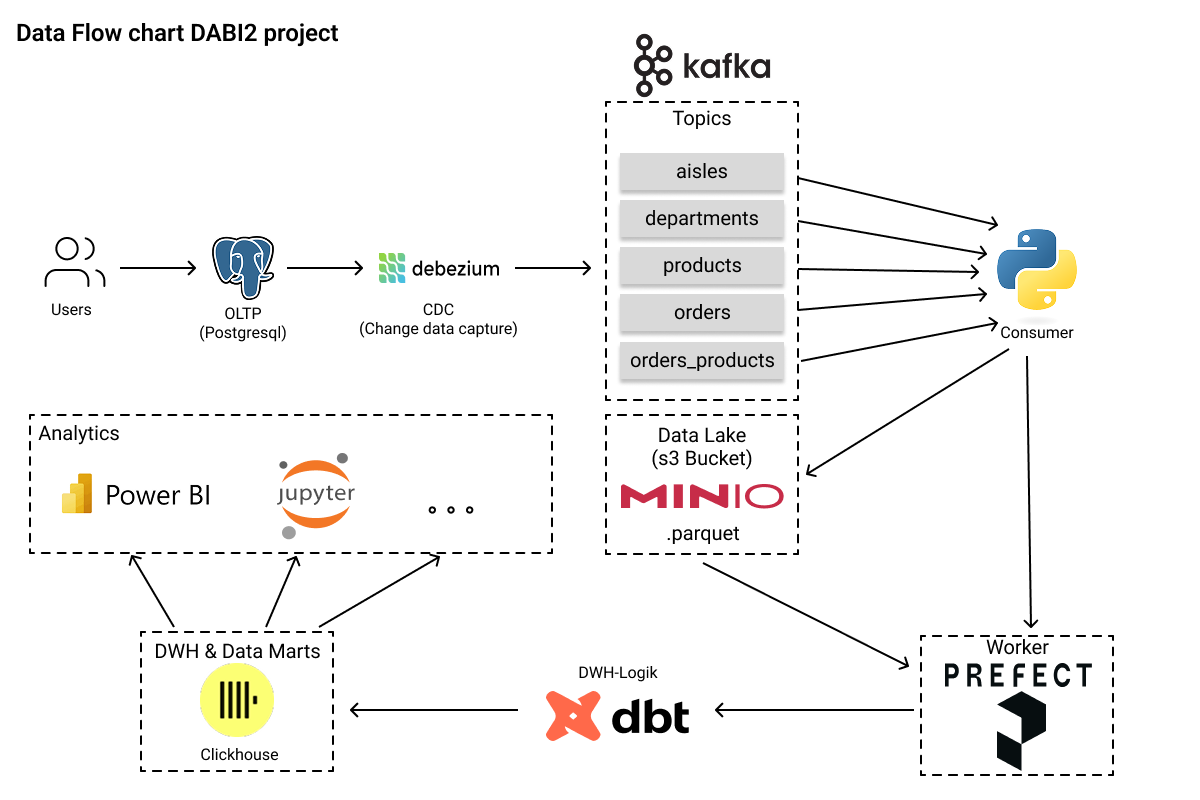
\includegraphics[width=\textwidth]{datenfluss.png}
    \caption{Konzeptioneller Datenfluss der entworfenen Architektur}
    \label{fig:architektur_diagramm}
\end{figure}

Dieser Aufbau stellt sicher, dass das OLTP-System minimal belastet wird, während die Analysten auf aktuellen und für ihre Zwecke optimierten Daten arbeiten können. Im Folgenden wird die Wahl der Technologie für jede dieser Stufen erläutert.

\subsection{Begründung der Technologie-Auswahl}
\label{sec:technologie_auswahl}

\subsection{Quellsystem und Datenerfassung: PostgreSQL \& Debezium}
\label{subsec:postgres_debezium}

Das Quellsystem ist eine \textbf{PostgreSQL}-Datenbank, die als operatives OLTP-System für den fiktiven Lieferdienst dient. Um die darin enthaltenen Daten für Analysezwecke abzugreifen, wurde bewusst auf eine direkte Abfrage der Tabellen verzichtet. Stattdessen kommt \textbf{Change Data Capture (CDC)} mithilfe von \textbf{Debezium} zum Einsatz.

Die Entscheidung für diesen Ansatz gründet sich auf mehrere Vorteile:
\begin{itemize}
    \item \textbf{Minimale Systemlast:} Debezium liest direkt aus dem Write-Ahead Log (WAL) von PostgreSQL. Dieser Mechanismus belastet die produktive Datenbank weitaus geringer als regelmäßige, komplexe \texttt{SELECT}-Abfragen.
    \item \textbf{Echtzeitnahe Daten:} Jede Datenänderung (INSERT, UPDATE, DELETE) wird als separates Ereignis erfasst und sofort weitergeleitet. Dies ermöglicht eine hohe Aktualität der Daten im analytischen System.
    \item \textbf{Vollständige Abdeckung:} Im Gegensatz zu Abfragen, die nur den aktuellen Zustand erfassen, protokolliert CDC auch Löschvorgänge, was für die korrekte Abbildung der Historie im Data Warehouse unerlässlich ist.
\end{itemize}
Debezium wurde als Werkzeug gewählt, da es ein etablierter Open-Source-Standard ist und nahtlos als Kafka-Connect-Source-Connector fungiert, was den direkten Anschluss an die Streaming-Plattform ermöglicht.

\subsection{Streaming-Plattform: Apache Kafka}
\label{subsec:kafka}

Als zentrales Nervensystem der Architektur dient \textbf{Apache Kafka}. Alle von Debezium erfassten Änderungsereignisse werden in Kafka-Topics publiziert. Die Wahl fiel auf Kafka aus folgenden Gründen:
\begin{itemize}
    \item \textbf{Entkopplung:} Kafka entkoppelt die datenproduzierenden Systeme (hier: Debezium) von den datenkonsumierenden Systemen (z.B. der Data-Lake-Lader). Neue Konsumenten können hinzugefügt werden, ohne die Produzenten zu beeinflussen.
    \item \textbf{Persistenz und Wiederholbarkeit:} Kafka speichert die Ereignisse für einen konfigurierbaren Zeitraum. Dies macht den Datenstrom wiederholbar (``replayable''). Fällt ein Konsument aus, kann er nach dem Neustart genau dort weiterarbeiten, wo er aufgehört hat. Muss die Logik eines Konsumenten geändert werden, kann er den gesamten Datenstrom von Neuem verarbeiten.
    \item \textbf{Skalierbarkeit und Ausfallsicherheit:} Als verteiltes System ist Kafka horizontal skalierbar und hochverfügbar, was es zu einer robusten Lösung für kritische Dateninfrastrukturen macht.
\end{itemize}

\subsection{Rohdatenspeicherung: Minio als Data Lake}
\label{subsec:minio}

Die aus Kafka konsumierten Rohdaten werden zunächst unverändert in einem Data Lake abgelegt. Als Technologie wurde ein S3-kompatibler Objektspeicher in Form von \textbf{Minio} gewählt. Die Daten werden im \textbf{Parquet-Format} gespeichert.
\begin{itemize}
    \item \textbf{Langlebigkeit und Kosten:} Ein Data Lake bietet eine kostengünstige Möglichkeit, große Mengen an Rohdaten dauerhaft zu speichern. Er dient als persistente \textit{Source of Truth} für alle nachgelagerten Transformationsprozesse.
    \item \textbf{Schema-on-Read:} Der Data Lake erzwingt kein bestimmtes Schema. Dies bietet die Flexibilität, die Rohdaten für verschiedene, auch zukünftige, Anwendungsfälle zu nutzen.
    \item \textbf{S3-Kompatibilität:} Die S3-API ist der De-facto-Standard für Objektspeicher. Die Wahl von Minio stellt die Kompatibilität mit einer riesigen Anzahl von Werkzeugen im Data-Engineering-Ökosystem sicher.
    \item \textbf{Effizientes Spaltenformat:} Parquet ist ein spaltenbasiertes Dateiformat. Analytische Abfragen, die oft nur einer Teilmenge der Spalten einer Tabelle benötigen, sind auf diesem Format deutlich performanter als auf zeilenbasierten Formaten wie CSV oder JSON.
\end{itemize}

\subsection{Transformation und Modellierung: dbt}
\label{subsec:dbt}

Für die Transformation der Rohdaten aus dem Data Lake in ein sauberes, strukturiertes Datenmodell im Data Warehouse wird \textbf{dbt (data build tool)} eingesetzt. dbt wurde gewählt, weil es den Transformationsprozess professionalisiert:
\begin{itemize}
    \item \textbf{SQL als einzige Sprache:} Analysten können komplexe Transformationspipelines allein mit SQL-Kenntnissen erstellen. Die Logik bleibt verständlich und zugänglich.
    \item \textbf{Software-Engineering-Prinzipien:} dbt bringt Konzepte wie Versionierung (via Git), Modularisierung (über wiederverwendbare Modelle), Dokumentation und automatisierte Tests in den Analyseprozess. Dies erhöht die Qualität und Wartbarkeit der Datenmodelle enorm.
    \item \textbf{Entkopplung von der Orchestrierung:} dbt kümmert sich ausschließlich um die SQL-zu-SQL-Transformation. Die Ausführung der dbt-Jobs wird von einem externen Werkzeug wie Prefect angestoßen.
\end{itemize}

\subsection{Data Warehouse: ClickHouse}
\label{subsec:clickhouse}

Als Zieldatenbank für die aufbereiteten, analytischen Daten dient \textbf{ClickHouse}. Die Entscheidung für dieses hochperformante, spaltenorientierte Datenbanksystem wurde aus folgenden Gründen getroffen:
\begin{itemize}
    \item \textbf{Performance und Skalierbarkeit:} ClickHouse ist für seine herausragende Abfragegeschwindigkeit bei analytischen Workloads bekannt. Als server-basiertes System ist es von Grund auf für Echtzeitanalysen auf sehr großen Datenmengen konzipiert und horizontal skalierbar. Dies schafft eine zukunftssichere Grundlage für wachsende Datenmengen und komplexe Anfragen.
    \item \textbf{Echtzeit-Fähigkeiten:} Eine besondere Stärke von ClickHouse sind die \textit{Materialized Views}, die es ermöglichen, Aggregationen und Transformationen automatisch und inkrementell durchzuführen, sobald neue Daten eintreffen. Dies ist ideal, um die aus dem Streaming-Prozess kommenden CDC-Events effizient in vor-aggregierte Analysemodelle zu überführen.
    \item \textbf{Konnektivität und Ökosystem-Integration:} ClickHouse lässt sich nahtlos in das bestehende Ökosystem integrieren. Es bietet offizielle Treiber für Python, ist vollständig kompatibel mit dbt (über den \texttt{dbt-clickhouse}-Adapter) und kann Daten direkt aus externen Quellen wie dem S3-basierten Data Lake (Minio) lesen.
\end{itemize}

\subsection{Workflow-Orchestrierung: Prefect}
\label{subsec:prefect}

Die Steuerung des gesamten Datenflusses, vom Konsumieren der Kafka-Nachrichten bis zum Anstoßen der dbt-Transformationen, wird durch \textbf{Prefect} orchestriert. Die Verwendung von Prefect war Teil der Aufgabenstellung und bietet entscheidende Vorteile:
\begin{itemize}
    \item \textbf{Zentrale Steuerung und Überwachung:} Alle Schritte der Pipeline werden als ein zusammenhängender Flow definiert, dessen Ausführung zentral überwacht werden kann.
    \item \textbf{Fehlerbehandlung und Wiederholbarkeit:} Prefect bietet robuste Mechanismen für Wiederholungsversuche bei Fehlern (Retries) und eine detaillierte Protokollierung, was die Fehlersuche erheblich vereinfacht.
    \item \textbf{Python-nativ:} Da Prefect auf Python basiert, können komplexe Logiken und die Integration verschiedenster Werkzeuge elegant in einem einzigen Framework umgesetzt werden.
\end{itemize}

%%%%%%%%%%%%%%%%%%%%%%%%%%%%%%%%%%%%%%%%%%%%%%%%%%%%%%%%%
% KAPITEL 4
%%%%%%%%%%%%%%%%%%%%%%%%%%%%%%%%%%%%%%%%%%%%%%%%%%%%%%%%%
\section{Technische Implementierung}
\label{chap:technische_implementierung}

Nachdem die grundlegende Infrastruktur steht, widmet sich dieses Kapitel den spezifischen Konfigurationen und Code-Implementierungen, die den Datenfluss von der Quelle bis ins Data Warehouse realisieren.

\subsection{Setup der Infrastruktur mit Docker Compose}
\label{sec:docker_compose_setup}

Die gesamte für das Projekt benötigte Infrastruktur wird mithilfe von Docker und Docker Compose aufgesetzt. Dieser Ansatz gewährleistet eine hohe Reproduzierbarkeit und Portabilität, da alle Dienste und ihre Abhängigkeiten in einer einzigen, deklarativen \texttt{docker-compose.yml}-Datei definiert sind. Dies vereinfacht nicht nur die Entwicklung, sondern stellt auch sicher, dass die gesamte Architektur konsistent auf unterschiedlichen Systemen ausgeführt werden kann.

Die \texttt{docker-compose.yml}-Datei definiert und konfiguriert insgesamt zwölf Services, die sich in drei Hauptkategorien einteilen lassen: die Kerndatenpipeline, die Anwendungs- und Orchestrierungsschicht sowie diverse Entwicklungs- und Monitoring-Werkzeuge.

\begin{enumerate}
    \item \textbf{Kerndatenpipeline:}
    \begin{itemize}
        \item \textbf{\texttt{db} (PostgreSQL):} Als operatives OLTP-System wird ein \texttt{timescale/timescaledb:latest-pg16}-Image verwendet. Entscheidend für die Anbindung an Debezium ist die Konfiguration \texttt{wal\_level=logical}, welche die Voraussetzung für das Change Data Capture darstellt.
        \item \textbf{\texttt{zookeeper} und \texttt{kafka}:} Diese beiden Dienste (\texttt{confluentinc/cp-zookeeper:7.3.2} und \texttt{confluentinc/cp-kafka:7.3.2}) bilden die zentrale Streaming-Plattform.
        \item \textbf{\texttt{kafka-connect}:} Hier kommt das \texttt{debezium/connect:2.1}-Image zum Einsatz. Dieser Service ist dafür verantwortlich, die Verbindung zur PostgreSQL-Datenbank herzustellen und die Datenänderungen in die Kafka-Topics zu publizieren.
        \item \textbf{\texttt{minio}:} Ein \texttt{minio/minio:latest}-Container dient als S3-kompatibler Objektspeicher und bildet die technische Grundlage für den Data Lake.
        \item \textbf{\texttt{cdc-lake-writer}:} Ein eigens entwickelter Service, der auf die Kafka-Topics lauscht und die eintreffenden CDC-Events als Parquet-Dateien im Minio Data Lake persistiert.
        \item \textbf{\texttt{clickhouse-server}:} Stellt den ClickHouse-Server bereit (z.B. \texttt{clickhouse/clickhouse-server:latest}), der als hochperformantes, spaltenorientiertes Data Warehouse für die von dbt transformierten Daten dient.
    \end{itemize}
    
    \item \textbf{Anwendungs- und Orchestrierungsschicht:}
    \begin{itemize}
        \item \textbf{\texttt{prefect} und \texttt{prefect-worker}:} Ein \texttt{prefecthq/prefect:3-latest}-Image startet den Prefect-Server zur Workflow-Verwaltung. Ein \textit{custom-built} \texttt{prefect-worker} führt die definierten Daten-Pipelines aus, inklusive der dbt-Transformationen, die auf ClickHouse zielen.
    \end{itemize}
    
    \item \textbf{Entwicklungs- und Monitoring-Werkzeuge:}
    \begin{itemize}
        \item \textbf{\texttt{akhq}:} Eine Web-Oberfläche zur einfachen Verwaltung und Überwachung des Kafka-Clusters und der Debezium-Konnektoren.
    \end{itemize}
\end{enumerate}

Die Stabilität des Systemstarts wird durch die gezielte Verwendung von \texttt{depends\_on} in Kombination mit \texttt{healthcheck}-Anweisungen sichergestellt. Dadurch wird gewährleistet, dass abhängige Dienste erst starten, wenn die darunterliegenden Services, wie die Datenbank oder Kafka, vollständig betriebsbereit sind. Persistente Daten, wie die der PostgreSQL-Datenbank oder des Minio Data Lakes, werden über benannte Docker-Volumes (\texttt{postgres\_data}, \texttt{minio\_data}) über den Lebenszyklus der Container hinaus gespeichert.

\subsection{Konfiguration des Debezium-Konnektors}
\label{sec:debezium_konfiguration}

Nachdem der \texttt{kafka-connect}-Dienst gestartet ist, wird der eigentliche Debezium-Konnektor für PostgreSQL über dessen REST-API konfiguriert. Dazu wird eine JSON-Payload an den \texttt{/connectors}-Endpunkt gesendet. Diese Konfiguration instruiert Debezium, welche Datenbank und welche Tabellen überwacht und wie die resultierenden Änderungsereignisse formatiert werden sollen.

Die zentrale Konfiguration ist zu finden unter (\texttt{src/prefect/config/debezium-pg-connector.json})

\subsection{Implementierung des Kafka-Consumers}
\label{sec:kafka_consumer}

Der \texttt{cdc-lake-writer}-Service ist eine in Python implementierte Anwendung, deren Aufgabe es ist, die von Debezium erzeugten CDC-Ereignisse aus Kafka zu konsumieren und als partitionierte Parquet-Dateien im Minio Data Lake abzulegen. Die Implementierung setzt auf die \texttt{confluent-kafka-python}-Bibliothek für die Kafka-Kommunikation und \texttt{pyarrow} für die Verarbeitung und Speicherung im Parquet-Format.

Die Kernlogik des Consumers ist eine Endlosschleife, die kontinuierlich Nachrichten aus allen relevanten Topics (via Topic-Pattern \texttt{cdc.oltp\_dabi.*}) abruft. Um die Entstehung vieler kleiner Dateien im Data Lake zu vermeiden, wird ein Batching-Mechanismus implementiert:

\begin{enumerate}
    \item \textbf{Sammeln im Puffer:} Jede eingehende Nachricht wird in einem \texttt{defaultdict}, dem \texttt{message\_buffer}, zwischengespeichert, der die Nachrichten nach ihrem Herkunfts-Topic gruppiert.
    
    \item \textbf{Zeitgesteuertes Schreiben:} Ein Schreibzyklus wird ausgelöst, wenn seit dem letzten erfolgreichen Schreibvorgang ein definiertes Zeitintervall (z.B. 60 Sekunden) verstrichen ist und sich Nachrichten im Puffer befinden.
    
    \item \textbf{Verarbeitung und Speicherung:} Innerhalb des Schreibzyklus (\texttt{process\_and\_write\_batches}) werden die Nachrichten für jedes Topic in ein Pandas DataFrame umgewandelt (\texttt{transform\_payloads\_to\_dataframe}). Anschließend werden in \texttt{prepare\_dataframe\_for\_parquet\_storage} Partitionierungsinformationen basierend auf dem Zeitstempel des Ereignisses extrahiert. Schließlich schreibt die Funktion \texttt{write\_dataframe\_to\_minio} das DataFrame als partitionierte Parquet-Datei in den Minio-Bucket, wobei eine Hive-ähnliche Verzeichnisstruktur wie \texttt{cdc\_events/orders/year=2025/month=06/day=27/orders\_timestamp.parquet} verwendet wird, um spätere, partitionsbasierte Abfragen zu beschleunigen.
    
    \item \textbf{Fehlertoleranz und Offset-Management:} Um Datenverlust zu verhindern, wird eine manuelle Commit-Strategie für die Kafka-Offsets verfolgt. Erst wenn der Schreibvorgang für alle Batches in einem Zyklus erfolgreich war, wird die \texttt{commit\_offsets}-Funktion aufgerufen, die Kafka signalisiert, dass diese Nachrichten erfolgreich verarbeitet wurden. Schlägt auch nur ein Schreibvorgang fehl, wird der Offset nicht verschoben. Die fehlgeschlagenen Nachrichten verbleiben im Puffer und werden im nächsten Zyklus erneut verarbeitet, was eine ,,At-least-once''-Liefergarantie sicherstellt.
    
    \item \textbf{Anstoßen der Downstream-Prozesse:} Nach einem erfolgreichen Schreibvorgang in Minio wird zudem die Funktion \texttt{trigger\_prefect\_dwh\_flow\_run\_sync} aufgerufen, um den nachgelagerten dbt-Transformationsprozess über Prefect zu starten.
\end{enumerate}

Diese Implementierung stellt ein robustes und fehlertolerantes Bindeglied zwischen der Echtzeit-Datenerfassung und dem Data Lake dar.

\subsection{Datentransformation mit dbt}
\label{sec:dbt_transformation}

Sobald die Rohdaten als Parquet-Dateien im Data Lake landen, beginnt der letzte Schritt der Pipeline: die Transformation der Rohdaten in ein sauberes, performantes und analysefreundliches dimensionales Modell im ClickHouse Data Warehouse. Dieser gesamte Prozess wird durch dbt gesteuert, dessen Ausführung wiederum von Prefect orchestriert wird.

\subsubsection{ELT-Prozess: Laden der Rohdaten aus dem Data Lake}
\label{sssec:elt_prozess}
Bevor dbt seine Transformationen ausführen kann, müssen die neuen Daten aus dem Minio Data Lake in das ClickHouse Data Warehouse geladen werden. Dieser Ladeschritt wird durch den Prefect-Flow \texttt{cdc\_minio\_to\_clickhouse\_flow} gesteuert und vollzieht sich in mehreren Schritten:
\begin{enumerate}
    \item \textbf{Dateien finden:} Der Task \texttt{find\_new\_files\_in\_minio} scannt das Staging-Verzeichnis im Minio-Bucket und erstellt eine Liste aller neuen, noch nicht verarbeiteten Parquet-Dateien.
    \item \textbf{Daten in ClickHouse laden:} Der zentrale Task \texttt{load\_files\_to\_clickhouse\_staging} iteriert über diese Dateiliste. Für jede Parquet-Datei verbindet er sich mit dem ClickHouse-Server und nutzt dessen native \texttt{s3}-Tabellenfunktion, um direkt auf den S3-Endpunkt von Minio zuzugreifen. Mittels eines Befehls wie \texttt{INSERT INTO cdc\_staging.raw\_table SELECT * FROM s3(...)} werden die Daten aus der Parquet-Datei direkt in die entsprechende rohe Staging-Tabelle in ClickHouse geladen.
    \item \textbf{dbt ausführen:} Nachdem alle neuen Daten in den rohen Staging-Tabellen in ClickHouse verfügbar sind, startet Prefect den Task \texttt{run\_dbt\_command\_runner}, der den Befehl \texttt{dbt build} ausführt. An diesem Punkt übernimmt dbt die Kontrolle über die weitere Transformation.
    \item \textbf{Dateien archivieren:} Nach einem erfolgreichen dbt-Lauf verschiebt der Task \texttt{archive\_processed\_files} die verarbeiteten Parquet-Dateien in ein Archivverzeichnis innerhalb von Minio, um eine erneute Verarbeitung zu verhindern.
\end{enumerate}
Dieser vorgeschaltete Ladeprozess stellt sicher, dass dbt immer auf den aktuellsten Rohdaten arbeitet, die seit dem letzten Lauf im Data Lake angekommen sind.

\subsubsection{dbt-Modellierungsstruktur}
\label{sssec:dbt_modellierung}
Das finale Datenmodell ist als klassisches Sternschema konzipiert (siehe Abbildung \ref{fig:dwh_schema}), um analytische Abfragen zu optimieren. Es besteht aus zwei zentralen Faktentabellen (\texttt{f\_orders}, \texttt{f\_order\_lines}) und den zugehörigen Dimensionstabellen (\texttt{dim\_product}, \texttt{dim\_user}, \texttt{dim\_date}).

\begin{figure}[h!]
    \centering
    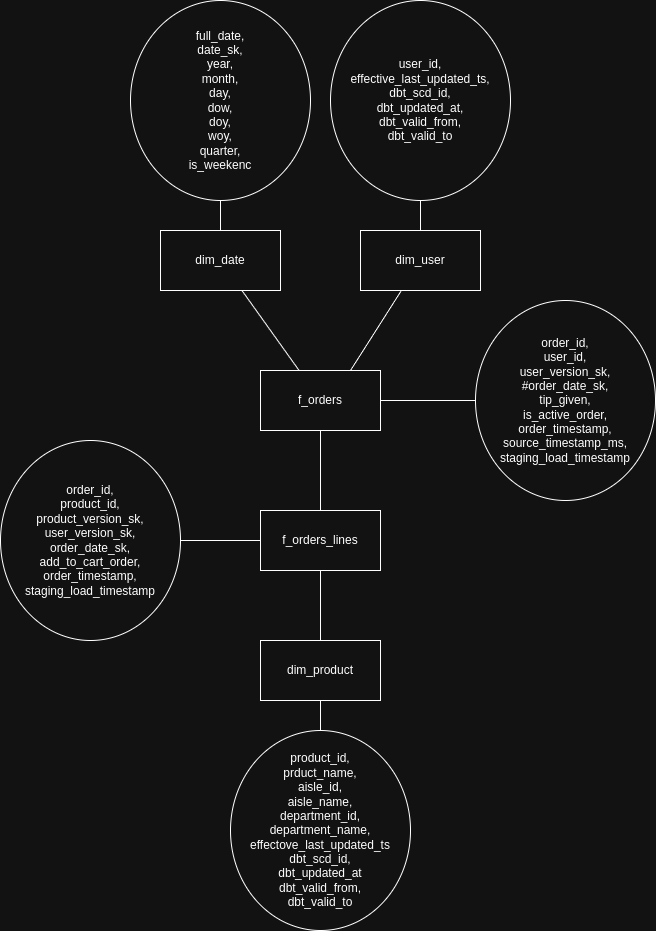
\includegraphics[width=\textwidth]{DWH_diagramm.png} % Bitte den Dateinamen anpassen
    \caption{Sternschema des finalen Data Warehouse-Modells.}
    \label{fig:dwh_schema}
\end{figure}

Das dbt-Projekt ist methodisch in mehrere logische Schichten unterteilt, was sich im gerichteten azyklischen Graphen (DAG) in Abbildung \ref{fig:dbt_dag} widerspiegelt. Dieser visualisiert die Abhängigkeiten zwischen den Modellen – von den Rohdatenquellen auf der linken Seite bis zu den finalen Fakten- und Dimensionstabellen auf der rechten Seite.

\begin{figure}[h!]
    \centering
    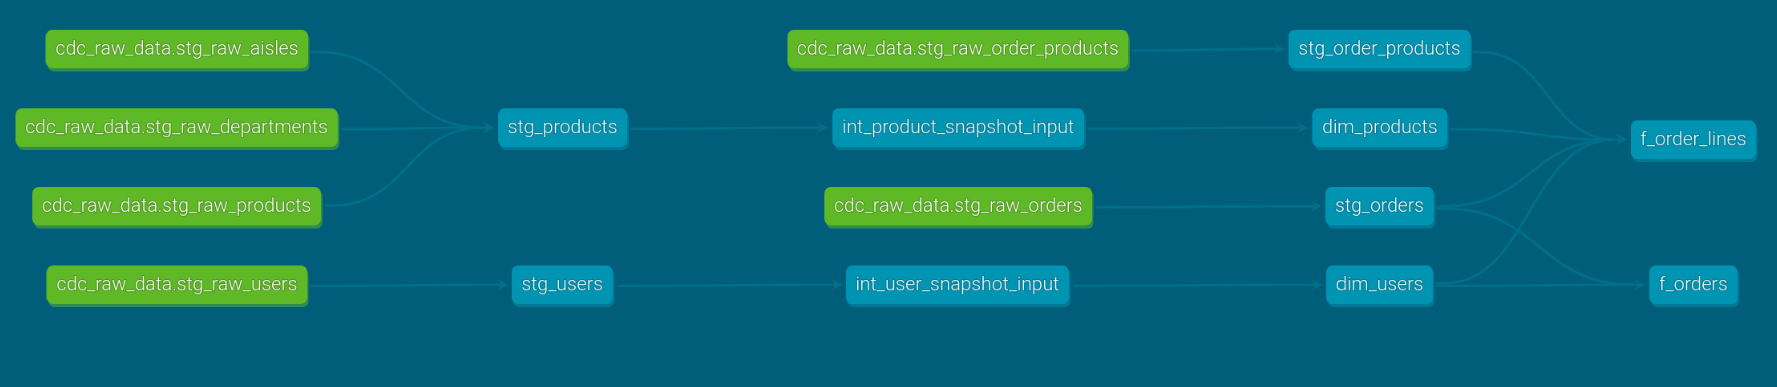
\includegraphics[width=\textwidth]{dbt_dag.png} % Bitte den Dateinamen anpassen
    \caption{dbt DAG der Transformationspipeline.}
    \label{fig:dbt_dag}
\end{figure}

Die Anbindung an die von Prefect geladenen Rohdaten wird über die \texttt{sources.yml}-Datei deklariert. Hier werden die rohen Staging-Tabellen als Quellen (\texttt{cdc\_staging}) definiert, auf die in den Staging-Modellen von dbt mittels der \texttt{\{\{ source(...) \}\}}-Funktion referenziert wird.

\subsubsection{Handhabung von Datenänderungen}
\label{sssec:dbt_datenhandling}
Ein Kernaspekt des Projekts ist die korrekte Verarbeitung von Datenhistorie und die effiziente Aktualisierung der Modelle. Hierfür werden zwei fortgeschrittene dbt-Konzepte eingesetzt:
\begin{itemize}
    \item \textbf{Slowly Changing Dimensions (SCD) mit Snapshots:} Für Dimensionen, deren Attribute sich über die Zeit ändern können (z. B. ein Benutzer oder ein Produkt), wird die \texttt{snapshot}-Funktionalität von dbt genutzt. Die Modelle im \texttt{snapshots}-Verzeichnis (z. B. \texttt{scd\_dim\_users.sql}) implementieren eine Typ-2-Historisierung. Als Strategie wurde \texttt{timestamp} gewählt. Diese weist dbt an, die Spalte \texttt{effective\_last\_updated\_ts} als Indikator für eine Änderung zu verwenden. Die Logik zur Ermittlung dieses Zeitstempels ist in \texttt{intermediate}-Modellen gekapselt, die mittels \texttt{GREATEST()} den jeweils neuesten Zeitstempel über mehrere zusammengehörige Tabellen ermitteln. dbt verwaltet dabei automatisch die Gültigkeitszeiträume (\texttt{dbt\_valid\_from}, \texttt{dbt\_valid\_to}) für jeden Datensatz. Die Faktentabellen wie \texttt{f\_orders.sql} führen anschließend einen point-in-time-korrekten Join durch, indem der Zeitstempel der Bestellung mit dem Gültigkeitszeitraum des Snapshots abgeglichen wird.

    \item \textbf{Effiziente Aktualisierung mit inkrementellen Modellen:} Die großen Faktentabellen (\texttt{f\_orders}, \texttt{f\_order\_lines}) sowie einige \texttt{intermediate}-Modelle sind als \texttt{materialized='incremental'} konfiguriert. Bei jeder nachfolgenden Ausführung sorgt die \texttt{\{\% if is\_incremental() \% \}}-Bedingung in der \texttt{WHERE}-Klausel dafür, dass nur neue oder geänderte Quelldaten verarbeitet werden, typischerweise basierend auf einem Ladezeitstempel. Dies reduziert die Laufzeit der Transformationen erheblich im Vergleich zu einem ständigen Neuaufbau.
\end{itemize}

\subsubsection{Initialisierung und Hilfsmodelle}
\label{sssec:dbt_hilfsmodelle}
\begin{itemize}
    \item \textbf{\texttt{seeds}:} Im Projekt wird die \texttt{seed}-Funktionalität für den initialen Ladevorgang (Initial Load) genutzt. Die CSV-Dateien im \texttt{seeds}-Verzeichnis enthalten den Anfangszustand der Dimensionstabellen. Durch das Laden dieser Daten mittels \texttt{dbt seed} wird sichergestellt, dass die allererste Version jedes Datensatzes in den \texttt{snapshot}-Tabellen einen korrekten und historisch validen \texttt{dbt\_valid\_from}-Zeitstempel erhält.

    \item \textbf{Utility-Modelle:} Das Modell \texttt{dim\_date.sql} ist ein klassisches Beispiel für eine generierte Dimensionstabelle. Anstatt eine statische Kalendertabelle zu pflegen, wird das Makro \texttt{dbt\_utils.date\_spine} aus dem \texttt{dbt-utils}-Paket verwendet, um dynamisch eine Kalendertabelle mit allen relevanten Datumsattributen zu erzeugen.
\end{itemize}
Durch die Kombination dieser Techniken entsteht ein Data Warehouse, das nicht nur performant und effizient aktualisiert wird, sondern auch eine vollständige und nachvollziehbare Historie der Geschäftsdaten abbildet.

\subsection{Orchestrierung der Gesamtpipeline mit Prefect}
\label{sec:prefect_orchestrierung}

Die Steuerung der gesamten ELT-Pipeline wird von Prefect orchestriert, das als zentrales Kontrollzentrum für die Automatisierung dient. Anstatt eines einzigen monolithischen Skripts wurde ein modularer Ansatz mit mehreren spezialisierten Flows implementiert. Die gesamte Orchestrierung wird durch ein zentrales Worker-Skript (\texttt{run\_worker.py}) initialisiert und verwaltet, das beim Start des \texttt{prefect-worker}-Containers ausgeführt wird.

\subsubsection{Deployment und intelligentes Bootstrapping}
\label{subsec:prefect_bootstrapping}

Das \texttt{run\_worker.py}-Skript ist für das Bootstrapping der gesamten Umgebung verantwortlich. Seine Aufgaben sind:
\begin{enumerate}
    \item \textbf{Work Pool erstellen:} Es stellt sicher, dass ein Prefect Work Pool namens \texttt{dabi2} existiert, in dem die Flows ausgeführt werden können.
    
    \item \textbf{Deployments registrieren:} Das Skript registriert alle für das Projekt notwendigen Flows als Deployments auf dem Prefect-Server. Dazu gehören der \texttt{initial\_oltp\_load\_flow} für das einmalige Setup, der \texttt{activate\_debezium\_flow} zur separaten Aktivierung des Connectors und der \texttt{cdc\_minio\_to\_clickhouse\_flow} für die laufende Verarbeitung.
    
    \item \textbf{Intelligenter Start:} Eine Schlüsselfunktion ist die \texttt{check\_oltp\_database\_readiness}-Logik. Beim Start prüft das Skript, ob die OLTP-Datenbank bereits initial befüllt ist. Ist die Datenbank leer, wird automatisch ein Flow Run für den \texttt{initial\_oltp\_load\_flow} getriggert. Ist die Datenbank bereits befüllt, wird stattdessen der \texttt{activate\_debezium\_flow} angestoßen, um sicherzustellen, dass die CDC-Erfassung nach einem Neustart des Systems wieder aktiv ist.
    
    \item \textbf{Worker starten:} Schließlich startet das Skript einen \texttt{ProcessWorker}, der auf den Work Pool lauscht und die anstehenden Flow Runs ausführt.
\end{enumerate}

\subsubsection{Der einmalige Setup-Flow: \texttt{initial\_oltp\_load\_flow}}
\label{subsec:prefect_setup_flow}

Dieser Flow dient dazu, das gesamte System aus einem leeren Zustand heraus in einen betriebsbereiten Zustand zu versetzen. Er wird nur einmalig durch das Bootstrapping-Skript angestoßen. Seine Schritte sind sorgfältig sequenziert, um Datenkonsistenz zu gewährleisten (siehe Abbildung Z). % Ggf. Abbildungsreferenz anpassen
\begin{enumerate}
    \item \textbf{Initialisierung des DWH:} Zuerst wird \texttt{dbt seed} ausgeführt, um die statischen Dimensionstabellen im Data Warehouse zu erzeugen.
    
    \item \textbf{Initialisierung des OLTP:} Parallel dazu werden die Tabellen in der operativen PostgreSQL-Datenbank erstellt und die Quelldaten (z.B. aus CSV-Dateien) in die OLTP-Tabellen geladen.
    
    \item \textbf{Aktivierung von Debezium:} An einem kritischen Punkt während des Ladevorgangs wird der \texttt{activate\_debezium\_connector\_task} aufgerufen. Dies stellt sicher, dass die CDC-Erfassung beginnt, bevor die letzten transaktionalen Daten geschrieben werden, sodass keine Änderungen zwischen dem Ende des Batch-Loads und dem Start des Streamings verloren gehen.
    
    \item \textbf{Abschluss des Ladens:} Die restlichen Daten werden in die Faktentabellen des OLTP-Systems geladen.
\end{enumerate}

\begin{figure}[h!]
    \centering
    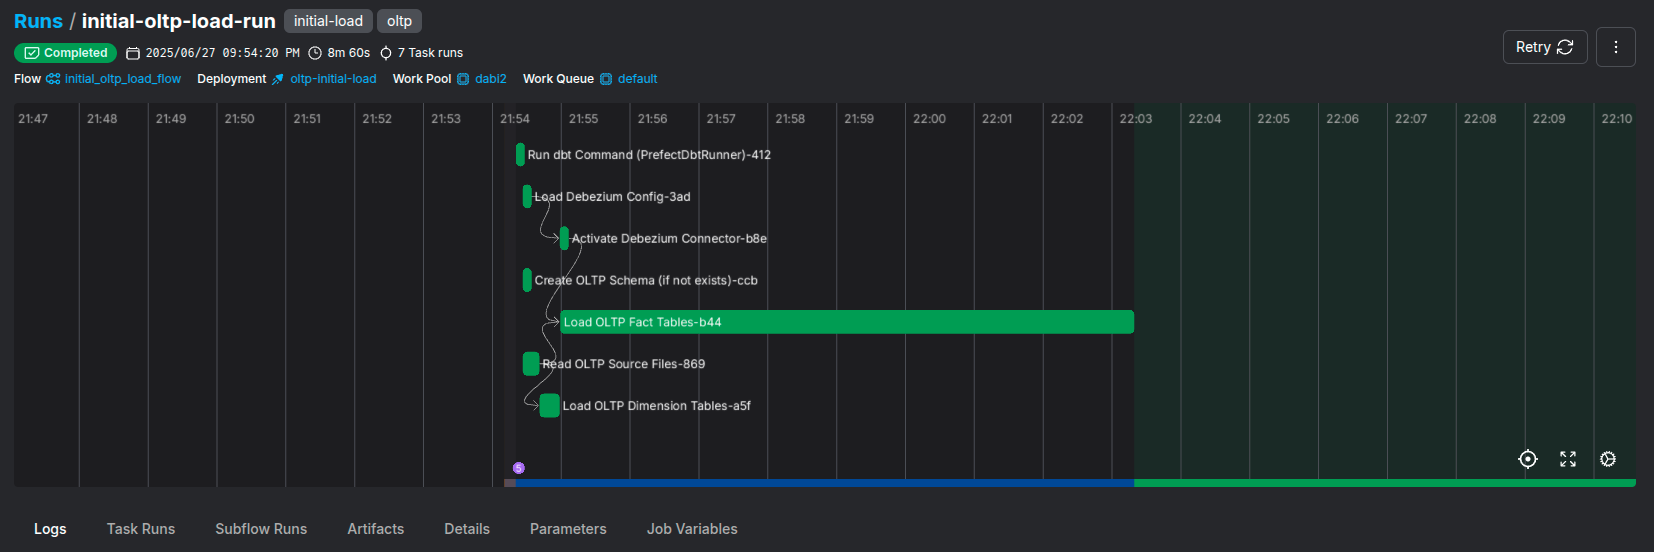
\includegraphics[width=\textwidth]{initial-flow.png} % Dateinamen des Screenshots anpassen
    \caption{Abhängigkeitsgraph des \texttt{initial\_oltp\_load\_flow} in der Prefect UI.}
    \label{fig:setup_flow}
\end{figure}

\subsubsection{Die wiederkehrende CDC-Pipeline: \texttt{cdc\_minio\_to\_clickhouse\_flow}}
\label{subsec:prefect_cdc_clickhouse_flow}

Dies ist der zentrale, operative Flow, der für die kontinuierliche Verarbeitung neuer Daten verantwortlich ist. Er wird durch den \texttt{cdc-lake-writer}-Service nach jedem erfolgreichen Schreibvorgang in Minio getriggert. Der Ablauf ist wie folgt (siehe Abbildung W): % Ggf. Abbildungsreferenz anpassen
\begin{enumerate}
    \item \textbf{Dateien im Data Lake finden (\texttt{find\_new\_files\_in\_minio}):} Der Flow beginnt mit dem Scannen des Staging-Verzeichnisses im Minio-Bucket nach neuen Parquet-Dateien. Sind keine neuen Dateien vorhanden, wird der Flow beendet.
    
    \item \textbf{Rohdaten in ClickHouse laden (\texttt{load\_files\_to\_clickhouse\_staging}):} Dieser Task lädt die gefundenen Dateien in die Staging-Tabellen in ClickHouse, wie in Abschnitt \ref{sssec:elt_prozess} beschrieben.
    
    \item \textbf{dbt-Transformationen ausführen (\texttt{run\_dbt\_command\_runner}):} Nach dem erfolgreichen Laden wird der Befehl \texttt{dbt build} gestartet, der alle definierten Modelle, Snapshots und Tests in der korrekten Reihenfolge ausführt.
    
    \item \textbf{Verarbeitete Dateien archivieren (\texttt{archive\_processed\_files}):} Nach einem erfolgreichen dbt-Lauf verschiebt dieser Task die verarbeiteten Dateien aus dem Staging- in ein Archivverzeichnis.
\end{enumerate}

\begin{figure}[h!]
    \centering
    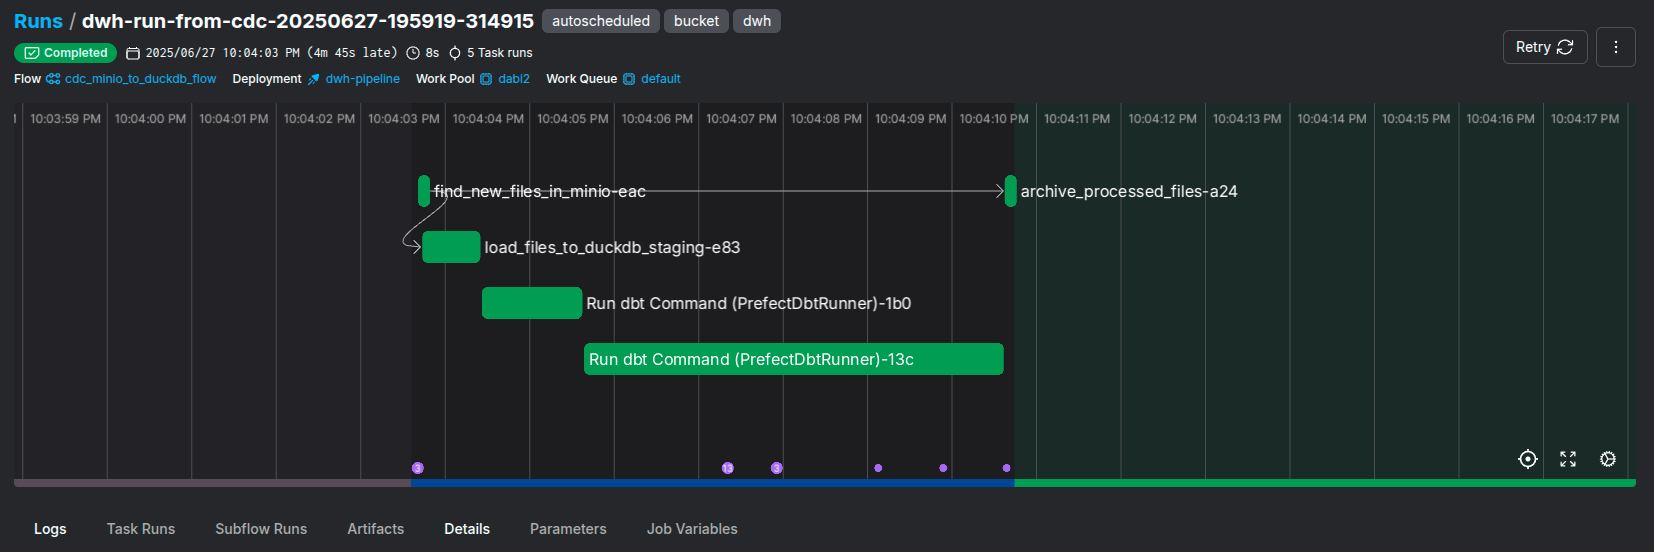
\includegraphics[width=\textwidth]{cdc-flow.png} % Dateinamen des Screenshots anpassen
    \caption{Abhängigkeitsgraph des \texttt{cdc\_minio\_to\_clickhouse\_flow} in der Prefect UI.}
    \label{fig:cdc_flow}
\end{figure}

Jeder dieser Schritte ist als Prefect-Task mit dem \texttt{@task}-Decorator implementiert, was die Nutzung von Features wie automatischen Wiederholungsversuchen (\texttt{retries=1}) und zentralisiertem Logging über den \texttt{get\_run\_logger()} ermöglicht. Durch diesen modularen Ansatz wird die komplexe Pipeline in logische, wiederverwendbare und überwachbare Prozesse zerlegt.

\section{Ergebnisse und Validierung}
\label{chap:ergebnisse}

Nach der Konzeption und technischen Implementierung der Datenpipeline in den vorherigen Kapiteln werden in diesem Kapitel die finalen Ergebnisse präsentiert. Es wird das im Data Warehouse entstandene Datenmodell detailliert beschrieben und anschließend validiert, indem gezeigt wird, wie es zur Beantwortung der ursprünglichen analytischen Fragestellung genutzt werden kann.

\subsection{Das finale Datenmodell im Data Warehouse}
\label{sec:finales_datenmodell}

Das Ergebnis der gesamten ELT-Pipeline ist ein sauberes, analysefreundliches Datenmodell im ClickHouse Data Warehouse, das nach den Prinzipien des Sternschemas aufgebaut ist (siehe Abbildung \ref{fig:dwh_schema}). Dieses Modell ist darauf optimiert, komplexe analytische Abfragen performant auszuführen und besteht aus den folgenden Kernkomponenten:

\begin{itemize}
    \item \textbf{Faktentabellen:} Sie enthalten die quantitativen Messwerte der Geschäftsprozesse.
    \begin{itemize}
        \item \textbf{\texttt{f\_orders}:} Die zentrale Faktentabelle, deren Granularität eine Zeile pro Bestellung ist. Sie enthält den Fremdschlüssel zum bestellenden Benutzer (\texttt{user\_version\_sk}), einen Fremdschlüssel zum Bestelldatum (\texttt{order\_date\_sk}) sowie die entscheidende Kennzahl, ob ein Trinkgeld gegeben wurde (\texttt{tip\_given}). Ein \texttt{is\_active\_order}-Flag, das aus dem CDC-Operationstyp abgeleitet wird, ermöglicht das logische Löschen von stornierten Bestellungen.
        \item \textbf{\texttt{f\_order\_lines}:} Diese Tabelle bildet die einzelnen Bestellpositionen ab und hat die Granularität ,eine Zeile pro Produkt pro Bestellung''. Sie verknüpft die Bestellungen mit den jeweiligen Produkten über die Fremdschlüssel \texttt{product\_version\_sk} und \texttt{user\_version\_sk}.
    \end{itemize}

    \item \textbf{Dimensionstabellen:} Sie beschreiben die ,,Wer''-, ,,Was''- und ,,Wann''-Aspekte der Geschäftsprozesse.
    \begin{itemize}
        \item \textbf{\texttt{dim\_users} und \texttt{dim\_products}:} Diese beiden Dimensionen werden als Slowly Changing Dimension (SCD) vom Typ 2 mittels dbt Snapshots verwaltet. Sie historisieren Änderungen an Benutzer- oder Produktdaten (z.B. eine Änderung des Produktnamens). Jede Zeile repräsentiert eine spezifische Version eines Benutzers oder Produkts mit einem eigenen Primärschlüssel (\texttt{dbt\_scd\_id}, der als Fremdschlüssel in den Faktentabellen dient) und einem Gültigkeitszeitraum. Dies ermöglicht point-in-time-korrekte Analysen.
        \item \textbf{\texttt{dim\_date}:} Eine generierte Kalenderdimension, die eine Fülle von Datumsattributen (Tag, Woche, Monat, Quartal, Wochentag, etc.) für jede Bestellung bereitstellt und so zeitbasierte Analysen stark vereinfacht.
    \end{itemize}
\end{itemize}

Dieses klar strukturierte Modell ermöglicht es Analysten, komplexe Abfragen zu formulieren, ohne sich mit der Komplexität der Rohdaten oder aufwändigen Joins über normalisierte Tabellen auseinandersetzen zu müssen.

\subsection{Validierung des Anwendungsfalls}
\label{sec:validierung}

Um die Praxistauglichkeit des Datenmodells zu demonstrieren, wird der initiale Anwendungsfall – die Analyse des Trinkgeldverhaltens – aufgegriffen. Ein Analyst möchte beispielsweise die monatliche Trinkgeld-Rate ermitteln, um Trends oder saisonale Muster zu erkennen. Mit dem finalen Datenmodell lässt sich diese Frage durch eine einfache SQL-Abfrage beantworten:

\begin{verbatim}
SELECT
    d.year,
    d.month,
    COUNT(f.order_id) AS total_orders,
    SUM(CASE WHEN f.tip_given THEN 1 ELSE 0 END) AS orders_with_tip,
    (SUM(CASE WHEN f.tip_given THEN 1 ELSE 0 END) * 1.0 / COUNT(f.order_id)) * 100 AS tip_rate_percent
FROM
    f_orders f
JOIN
    dim_date d ON f.order_date_sk = d.date_sk
GROUP BY
    1, 2
ORDER BY
    1, 2;
\end{verbatim}

Diese Abfrage verknüpft die Faktentabelle \texttt{f\_orders} mit der Datumsdimension \texttt{dim\_date}, um die Bestelldaten auf Monatsbasis zu aggregieren. Sie berechnet die Gesamtzahl der Bestellungen, die Anzahl der Bestellungen mit Trinkgeld und leitet daraus die prozentuale Trinkgeld-Rate ab. Die Einfachheit und Lesbarkeit dieser Abfrage validiert den Erfolg des dimensionalen Modells: Komplexe Zusammenhänge sind in einer einfachen, performanten Struktur abgebildet, die es Analysten ermöglicht, sich auf die Beantwortung von Geschäftsfragen zu konzentrieren, anstatt Zeit mit aufwändiger Datenaufbereitung zu verbringen.

\section{Fazit und Ausblick}
\label{chap:fazit}

Diese Projektarbeit hatte zum Ziel, eine moderne und robuste Datenplattform zu konzipieren und prototypisch zu implementieren, die es ermöglicht, operative Daten für analytische Zwecke zu nutzen, ohne die Stabilität des Quellsystems zu gefährden. Dieses abschließende Kapitel fasst die Ergebnisse der Arbeit zusammen, reflektiert die aufgetretenen Herausforderungen und deren Lösungen und gibt einen Ausblick auf mögliche zukünftige Erweiterungen.

\subsection{Zusammenfassung der Arbeit}
\label{sec:fazit_zusammenfassung}

Ausgehend von der Notwendigkeit, Fachanalysten eine performante und flexible Datenbasis für die Entwicklung von Vorhersagemodellen zur Verfügung zu stellen, wurde eine an die Kappa-Architektur angelehnte, streaming-basierte Dateninfrastruktur entworfen. Durch den Einsatz von Change Data Capture (CDC) mit Debezium werden Datenänderungen aus der operativen PostgreSQL-Datenbank ressourcenschonend und in Echtzeit erfasst und über eine Apache Kafka Streaming-Plattform verteilt.

Die weitere Verarbeitung folgt einem modernen ELT-Ansatz: Die Rohdaten werden zunächst unverändert in einem S3-kompatiblen Data Lake (Minio) persistiert. Von dort aus lädt ein durch Prefect orchestrierter Prozess die Daten in ein ClickHouse Data Warehouse. Die finale Transformation und Modellierung der Daten in ein analysefreundliches Sternschema wird von dbt übernommen. Hierbei kommen fortgeschrittene Techniken wie die Historisierung von Dimensionen mittels dbt Snapshots (SCD Typ 2) und die effiziente Aktualisierung von Faktentabellen durch inkrementelle Modelle zum Einsatz.

Das Ergebnis ist ein voll funktionsfähiger Prototyp einer Datenplattform, die eine klare Trennung zwischen operativen und analytischen Systemen gewährleistet. Sie stellt den Analysten ein dimensionales Datenmodell zur Verfügung, das nicht nur aktuell, sondern auch vollständig historisiert ist und somit komplexe point-in-time-Analysen ermöglicht.

\subsection{Reflexion und Herausforderungen}
\label{sec:fazit_reflexion}

Im Laufe des Projekts traten verschiedene technische und konzeptionelle Herausforderungen auf, für die pragmatische Lösungen gefunden wurden:

\begin{itemize}
    \item \textbf{Komplexität des Technologie-Stacks:} Die Orchestrierung von über zehn verschiedenen Diensten stellt eine erhebliche Komplexität dar. Die Verwendung von Docker Compose in Kombination mit expliziten \texttt{depends\_on}-Beziehungen und \texttt{healthcheck}-Anweisungen erwies sich als entscheidend, um einen stabilen und reproduzierbaren Start der gesamten Infrastruktur zu gewährleisten.

    \item \textbf{Bootstrapping des Gesamtsystems:} Eine zentrale Frage war, wie der initiale Zustand des Systems (leere Datenbank) vom laufenden Betrieb unterschieden werden kann. Die Lösung war ein intelligentes Bootstrapping-Skript im Prefect-Worker, das beim Start den Zustand der Zieldatenbank prüft und je nach Ergebnis entweder den einmaligen initialen Lade-Flow oder den regulären Debezium-Aktivierungs-Flow anstößt.

    \item \textbf{Konsistenz und Datenverlust:} In einem asynchronen System wie diesem ist die Sicherstellung, dass keine Daten verloren gehen, von größter Bedeutung. Dies wurde durch eine manuelle Commit-Strategie im Kafka-Consumer gelöst. Ein Offset wird erst dann committet, wenn die entsprechenden Daten erfolgreich in den Data Lake geschrieben wurden. In Kombination mit einem Archivierungsmechanismus für verarbeitete Dateien wird so eine ,,At-least-once''-Verarbeitungsgarantie realisiert.

    \item \textbf{Historisierung von Dimensionen:} Die korrekte Abbildung von Attributänderungen in Dimensionen (SCD Typ 2) ist eine klassische Herausforderung im Data Warehousing. Anstatt die komplexe Logik manuell zu implementieren, wurde auf die \texttt{snapshot}-Funktionalität von dbt zurückgegriffen. Die Herausforderung verlagerte sich somit auf die korrekte Definition des ,,effektiven Änderungsdatums'' (\texttt{effective\_last\_updated\_ts}) in vorgelagerten \texttt{intermediate}-Modellen, was durch die \texttt{GREATEST()}-Funktion über mehrere relevante Quelltabellen gelöst wurde.
\end{itemize}

\end{document}